\documentclass{article}

\usepackage{listings}
\usepackage{xcolor}
\usepackage{courier}
\usepackage{graphicx}
\usepackage{float}
\usepackage[hidelinks]{hyperref}
\usepackage{caption}
\captionsetup[table]{name=جدول}
\usepackage{indentfirst}
%\usepackage{float}

\usepackage{xepersian}
\settextfont{HMXZar}
\setdigitfont{Times New Roman}

\definecolor{lightgray}{gray}{0.95}

\lstset{
basicstyle=\ttfamily,
backgroundcolor=\color{lightgray},
numbers=left,
tabsize=4,
frame=tblr,
breaklines=true, 
captiondirection=RTL
}
\renewcommand\lstlistingname{\rl{کد}}

\title{راهنمای استفاده از \lr{uv2cnf}\\
\lr{(Upgraded CNF to Verilog)}}
\date{تیر ۱۴۰۰}
\author{محمد (رها) مرادی شهمیری\\\lr{raham9619@gmail.com}}



\begin{document}
\pagenumbering{gobble}
\maketitle
\newpage
\rl{\tableofcontents}
\newpage

\pagenumbering{arabic}

\section{مقدمه}
نرم‌افزار \lr{uv2cnf} ابزاری برای تولید نمایش cnf مناسب برای دیباگ مدارات ترکیبی از روی توصیف سطح گیت به زبان وریلاگ است. 
برای استفاده از آن به کتابخانه‌ای با فرمت \lr{\textit{cnflib}} حاوی سلول‌های استاندارد استفاده‌شده در طرح نیاز است. علاوه بر آن می‌توان 
یک فایل حاوی پاسخ‌های دلخواه با فرمت \lr{\textit{sol}} و نیز فایلی حاوی متغیرهای مشمول محدودیت تعداد (cardinality) ورودی داد تا در خروجی 
تولیدشده به طور خودکار محدودیت‌های آن‌ها نیز اعمال شود. توصیف این فرمت‌ها در قسمت \ref{usage} خواهد آمد. 

\subsection{چرا \lr{uv2cnf}؟}

برای دیباگ مدارات سطح گیت روش‌های مختلفی وجود دارد که یکی از آن‌ها افزودن مالتی‌پلکسر به خروجی گیت‌های مشکوک (suspect) و پیداکردن مقادیر ورودی برای بیت انتخاب آن‌هاست که امکان تولید خروجی درست را فراهم کنند. به عبارت دیگر، در این روش معادله‌ی باینری نوشته می‌شود که با حل آن به وسیله‌ی SAT solver مشخص می‌شود چه گیت‌هایی باید تغییر کنند تا مدار خروجی مطلوب را تولید کند. توصیف سطح گیت بسیاری از مدارهای واقعی بزرگ بوده و اضافه‌کردن مالتی‌پلکسرها باعث بزرگتر شدن آن‌ها نیز می‌شود. از طرفی برای بررسی هر گیت دو ورودی به ۲ تا ۴ جمله در معادله‌ی باینری نیاز است. واضح است که تولید دستی چنین معادله‌ای بسیار زمان‌بر و مستعد خطاست. به همین دلیل نیاز به ابزارهایی‌ست که به شکل خودکار مراحل دیباگ را انجام دهند. 

در تمرین کامپیوتری ۳ درس Verification ارائه‌شده در ترم بهار ۱۳۹۹-۱۴۰۰ [cite] به این منظور از ابزاری به نام Verilog2CNF استفاده شد که تبدیل توصیف سطح گیت به معادله‌ی باینری را به شکل خودکار انجام می‌داد، اما محدودیت‌هایی داشت، از جمله این که افزودن مالتی‌پلکسرها به مدار به عهده‌ی کاربر بود و کارکرد ابزار نیز وابسته به کتابخانه‌ی \textit{gtech} بود. برای رفع مورد اول در حل همان تمرین برنامه‌ی \textit{insert\_gate.py} توسط نگارنده نوشته شد [cite]. در ادامه، در این کار سعی شده تا با برنامه‌ی \lr{uv2cnf} محدودیت دوم نیز برداشته شده و امکان جایگزینی آسان کتابخانه‌های دیگر به جای gtech فراهم شود. در این گزارش به نحوه‌ی استفاده از این ابزار و نوشتن فایل‌های لازم برای کار با آن پرداخته می‌شود. با وجود این که برای استفاده از تمامی قابلیت‌های این ابزار ممکن است نیاز به نوشتن ۳ فایل مختلف باشد، نگارنده بر این باور است که به دلیل استفاده از نام نت‌های (net) اصلی به جای شماره‌ی متغیرهای cnf انجام این کار بسیار آسان‌تر و کم‌خطاتر و تفسیر خروجی حاصل برای کاربر انسانی بسیار آسان‌تر خواهد بود. 

امید است با افزودن قابلیت‌هایی مانند خواندن فایل‌های استاندارد \lr{.lib} و تفسیر خودکار خروجی SAT solver در نهایت امکان خودکارسازی کامل فرآیند دیباگ مدارات ترکیبی سطح گیت با استفاده از این ابزار فراهم شود. 

\subsection{اقدامات بعدی}
قصد بر این بود که پشتیبانی از فرمت استاندارد لیبرتی \lr{(\textit{liberty})} از اولین نسخه وجود  داشته باشد، اما فرمت لیبرتی تابع منطقی متناظر با 
هر خروجی را به شکل یک تابع (function) و با استفاده از عملگرهای منطقی به نحوی نمایش می‌دهد که در صورتی که پیچیدگی تابع زیاد باشد، مثلا از پرانتزهای 
متعدد در آن استفاده شود، برای تبدیل آن به نمایش cnf نیاز به تعریف تعدادی سیم (wire) واسط خواهد بود که ورود آن‌ها به معادله، دیباگ را پیچیده خواهد کرد. 
به همین دلیل فعلا از پیاده‌سازی کامل این قابلیت صرف نظر شد. همچنین از آن‌جا که این ابزار در حال توسعه است، پشتیبانی آن از دستور وریلاگ بسیار محدود 
است. به طور خاص انتظار می‌رود که در ویرایش‌های بعدی و هم‌زمان با پشتیبانی از تابع‌های فرمت لیبرتی، پشتیبانی از \lr{assign statement}های وریلاگ نیز 
اضافه شود، چرا که نحوه‌ی پردازش و سنتز آن‌ها شبیه به هم است. 

\section{شروع به کار}
در این قسمت کلیت روش استفاده از \lr{uv2cnf} با استفاده از یک مثال ساده بررسی می‌شود. مدار مورد استفاده در این مثال از تمرین کامپیوتری شماره ۳ کلاس Verification دکتر علیزاده برداشته شده است [cite]. در قدم اول یک مدار سطح گیت به توصیف cnf تبدیل شده و روش تبدیل و خروجی تولیدشده بررسی می‌شود. در ادامه با افزودن محدودیت‌های بیشتر معادله‌ی لازم برای دیباگ مدار تولید شده، مدار دیباگ‌شده بررسی خواهد شد. در این قسمت از minisat به عنوان \lr{SAT solver} استفاده شده است [cite]. 

\subsection{تئوری عملکرد}

روشی که برای دیباگ مدارات سطح گیت در این ابزار پیاده شده، تولید معادله‌ای باینری‌ست که با حل آن مشخص شود خروجی کدام گیت "غلط" است. در ادامه می‌توان با تغییر این گیت خروجی را تصحیح کرد. 

برای هر گیت می‌توان معادله‌ای نوشت که در صورت عملکرد درست آن گیت خروجی آن ۱ وگرنه ۰ شود. به عنوان مثال برای گیت NAND دو ورودی می‌توان گفت: 
\begin{flushleft}
\lr{$ (W = (AB)') \rightarrow \{(W = 0: (A = 1)(B = 1))(W = 1: (A = 0) + (B = 0))\} $}

\lr{$ (W = 0: (A = 1)(B = 1)) \rightarrow (W + AB) = (W + A)(W + B) $}

\lr{$ W = 1: (A = 0) + (B = 0): (W' + A' + B') $}
\end{flushleft}

و معادله‌ی حاصل به شکل \ref{eq:nand} درمی‌آید.

\begin{flushleft}\lr{\begin{equation} \label{eq:nand}
f(W,A,B) = (W + A)(W + B)(W' + A' + B')
\end{equation}}\end{flushleft}

برای بررسی صحت این معادله، جدول صحت آن در  \ref{tbl:nand} آمده است. مشاهده می‌شود که خروجی تابع \lr{$f(A,B,W)$} برابر ۱ است اگر و تنها اگر رابطه‌ی \lr{$W=(AB)'$} برقرار باشد. 

\lr{\begin{table}[!htb]\begin{center}
\rl{\caption{جدول صحت معادله‌ی \ref{eq:nand}}
\label{tbl:nand}}
\begin{tabular}[c]{c|c|c|c}
\textbf{A} & \textbf{B} & \textbf{W} & \lr{\textbf{f(A, B, W)}}\\
\hline
0 & 0 & 0 & 0\\
0 & 0 & 1 & 1\\
0 & 1 & 0 & 0\\
0 & 1 & 1 & 1\\
1 & 0 & 0 & 0\\
1 & 0 & 1 & 1\\
1 & 1 & 0 & 1\\
1 & 1 & 1 & 0\\
\end{tabular}
\end{center}\end{table}}

برای توابع رایج دیگر، و به طور کلی هر تابع بولین، می‌توان معادلات مشابهی را بین ورودی‌ها و خروجی نوشت. برای به دست آوردن معادله‌ی یک مدار کافی‌ست معادله‌ی تک‌تک اجزای آن نوشته و با هم AND منطقی شوند. بدین ترتیب معادله‌ای به دست می‌آید که اگر به ازای یک ورودی دلخواه خروجی آن برابر ۱ شود، کارکرد مدار درست، وگرنه نادرست، خواهد بود. نحوه‌ی استفاده از این معادلات برای دیباگ مدار از حوصله‌ی این مقاله خارج است.  

\subsection{فرمت کتابخانه‌ی سلول‌ها}
با توجه به این که دیباگ در این روش در سطح گیت و کاملا مبنی بر ساختار انجام می‌شود، بدیهی‌ست که باید از مدار سنتزشده تا سطح گیت استفاده شود. چنین مدارهایی معمولا پیچیده‌تر از آن هستند که امکان تولید معادله‌ی آن‌ها به شکل دستی وجود داشته باشد و نیاز به استفاده از ابزارهای خودکار است. ابزار استفاده‌شده باید توانایی استفاده از کتابخانه‌ی استانداردی که مدار بر اساس آن سنتز شده، داشته باشد. در \lr{uv2cnf} این امکان فراهم شده است. 

برای تولید معادله‌ی cnf متناظر با یک گیت نیاز به نام آن گیت، فهرست ورودی‌ها و خروجی‌های آن، و معادله‌ی گیت بر حسب نام ورودی‌ها و خروجی‌هاست. با استفاده از نام گیت نگاشت آن به گیت‌های استفاده‌شده در توصیف سطح گیت مشخص شده و با استفاده از نام ورودی‌ها و خروجی‌ها، نام نت‌های مدار به نام پورت‌های گیت نگاشته می‌شود. یک فرمت پرکاربرد برای چنین روابطی فرمت لیبرتی (\lr{\textit{liberty}}) [cite] است. در این فرمت اطلاعات بسیاری در مورد هر سلول را می‌توان ذخیره کرد؛ ولی در این‌جا تنها به مواردی پرداخته می‌شود که برای تولید یک معادله به آن‌ها نیاز است. نمونه‌ی توصیف یک سلول با فرمت لیبرتی در کد \ref{lst:liberty} آمده است. [cite]

\begin{LTR}{\lstinputlisting[label={lst:liberty},caption={\rl{نمونه‌ی توصیف یک کتابخانه و یک سلول در فرمت لیبرتی}}]{samples/sample.lib}}\end{LTR}

قسمت‌های حاوی اطلاعات لازم عبارتند از: 
\begin{itemize}
\item \lr{(\rl{نام سلول}) cell}
\item \lr{(\rl{نام پین (متغیر)}) pin}
\item \lr{\rl{تابع منطقی خروجی بر حسب ورودی(ها)}: function <- pin}
\end{itemize}

برای توضیح کامل در مورد این فرمت به [cite] ارجاع داده می‌شود؛ اما به شکل مختصر، به جز نام سلول و نام پین که واضح هستند، فیلد function به شکل عبارتی بولین بر حسب نام ورودی‌ها نوشته می‌شود که در آن می‌توان از برخی عملگرهای رایج، پرانتز برای تعیین اولویت و برخی عناصر ترتیبی استفاده کرد. برای تبدیل سلول‌ها به فرم cnf باید عبارت بولین مذکور پردازش شده و رابطه‌ی جبری بین خروجی و ورودی‌های آن مشخص شود. با توجه به پیچیدگی که این پردازش در دیباگ ایجاد می‌کند، فرمتی ساده‌تر به نام \lr{\textit{cnflib}} تعریف شد که همین اطلاعات را ساده‌تر کد می‌کند. با این وجود، برای سازگاری با ابزارهای موجود، در ویرایش‌های بعدی امکان پردازش فایل لیبرتی نیز اضافه خواهد شد. 

جزئیات فرمت ارائه‌شده در قسمت \ref{section:cnflib} می‌آید. در این‌جا به این توضیح بسنده می‌شود که در فرمت cnflib نیز مشابه فرمت لیبرتی، هر سلول در قالب نام، نام پورت‌ها و نمایش تابع بولین ذخیره می‌شود، با این تفاوت که در این‌جا تابع در فرم cnf به نمایش درمی‌آید. 

\subsection{مثال استفاده از \lr{uv2cnf}}
در این بخش با استفاده از یک مثال عملی، استفاده از \lr{uv2cnf} نشان داده می‌شود. فایل‌های لازم برای اجرای این مثال در پوشه‌ی sample موجودند. 

\subsubsection{مدار ورودی سطح گیت}

\begin{LTR}{\lstinputlisting[label={lst:inputverilog},caption={\rl{گزیده‌ای از توصیف سطح گیت مدار باگ‌دار}}]{samples/comparator_debug_excerpt.v}}\end{LTR}

\subsubsection{کتابخانه‌ی cnflib}

\begin{LTR}{\lstinputlisting[label={lst:cnflib},caption={\rl{کتابخانه‌ی cnflib استفاده‌شده در این مثال}}]{samples/gtechsubset.cnflib}}\end{LTR}

\subsubsection{مثال اول: اجرای \lr{uv2cnf} و تولید خروجی}

با توجه به این که \lr{uv2cnf} به ازای هر ماژول یک زوج فایل cnf و map تولید می‌کند، بهتر است خروجی آن در یک پوشه قرار داده تا نظم آن حفظ شود. در این مثال پوشه‌ی \lr{output/} به عنوان پیشوند تولید خروجی به برنامه معرفی می‌شود تا خروجی تولیدشده در آن قرار بگیرد. بدین ترتیب با استفاده از فرمان زیر برنامه اجرا می‌شود: 

\begin{flushleft}
\lr{ \lstinline{./uverilog2cnf comparator_debug.v gtechsubset.cnflib output/ex1_ output/ex1_}}
\end{flushleft}

چند خط اول از دو فایل خروجی تولیدشده در کد \ref{lst:cnfex1} و \ref{lst:mapex1} آمده است. 

\begin{LTR}{\lstinputlisting[label={lst:cnfex1},caption={\rl{فایل cnf خروجی مثال اول}}]{samples/ex1_comparator_excerpt.cnf}}\end{LTR}
\begin{LTR}{\lstinputlisting[label={lst:mapex1},caption={\rl{فایل map خروجی مثال اول}}]{samples/ex1_comparator_excerpt.map}}\end{LTR}

در فایل cnf معادله‌ای قرار دارد که قابل حل با استفاده از SAT solver است. در فایل map نگاشتی از شماره‌ی متغیرهای فایل cnf به متغیرهای اصلی استفاده‌شده در طرح آمده که با استفاده از آن می‌توان نتایج را تفسیر کرد. اما جواب‌های این معادله چه معنایی دارند؟ 

با توجه به این که معادله‌ی نوشته‌شده، معادله‌ی صحت ساختار مدار بر حسب ورودی‌هاست، در صورتی که ورودی معتبری وجود داشته باشد که به ازای آن خروجی مدار برابر ۱ شود، معادله SAT بوده و SAT solver مثالی برای آن تولید می‌کند. بنابراین جواب حاصل عملا کاربردی ندارد. برای تولید خروجی مفید باید مثال‌هایی از عملکرد نادرست مدار بر معادله اعمالش شوند، به این شکل که به ازای هر مثال، ورودی متناظر با آن و خروجی \underline{درست} آن به شکل محدودیت‌هایی (constraint) به معادله اضافه شوند. در این مثال قبلا مالتی‌پلکسرهای لازم برای تصحیح عملکرد مدار اضافه شده و مدار به تعداد مثال‌های نقض تکرار شده است. بر این اساس در قسمت بعد با استفاده از \lr{uv2cnf} چند مثال نقض به شکل خودکار به معادله اضافه می‌شوند. 

\subsubsection {مثال دوم: افزودن خودکار مثال نقض}

در این مثال سه مثال نقض در دسترس است که در جدول \ref{tbl:ce} آمده‌اند. در ماژول مورد بررسی مدار در سه نسخه تکرار شده و نام سیگنال \textit{X} در سه نسخه {\lr{\textit{\_X\_1\_}}}، {\lr{\textit{\_X\_2\_}}} و {\lr{\textit{\_X\_3\_}}} است. 

\lr{\begin{table}[!htb]\begin{center}
\rl{\caption{مثال‌های نقض موجود}
\label{tbl:ce}}
\begin{tabular}[c]{c|c|c|c|c|c|c|c}
\textbf{A} & \textbf{B} & \textbf{L} & \textbf{E} & \textbf{G} & \textbf{A\_le\_B} & \textbf{A\_equal\_B} & \textbf{A\_greater\_B}\\
\hline
1 & 0 & 0 & 0 & 0 & 0 & 0 & 1\\
1 & 0 & 0 & 1 & 0 & 0 & 0 & 1\\
1 & 0 & 0 & 0 & 1 & 0 & 0 & 1\\
\end{tabular}
\end{center}\end{table}}

مثال‌های نقض فوق به شکل زیر در قالب فرمت \textit{sol} برای \lr{uv2cnf} تعریف می‌شوند. محتوای این فرمت نسبتا گویاست؛ توضیح بیشتر در قسمت \ref{section:sol} آمده است. 

\begin{LTR}{\lstinputlisting[label={lst:solex2},caption={\rl{تعریف مثال‌های نقض برای \lr{uv2cnf}}}]{samples/ex2_ec.sol}}\end{LTR}

با اعمال محدودیت مثال نقض فقط جواب‌هایی معتبر هستند که با اعمال مقادیر مناسب به ورودی‌های مالتی‌پلکسرها سبب می‌شوند خروجی مدار به ازای این ورودی‌ها تصحیح شود. هر سری از ورودی‌های اعمال‌شده به بیت انتخاب مالتی‌پلکسرها نشان‌دهنده‌ی یک روش برای تصحیح خروجی مدار به ازای مثال‌های نقض مورد بررسی است. برای روشن‌شدن این موضوع نخست با استفاده از \lr{uv2cnf} معادله‌ی باینری تولید شده و سپس با استفاده از minisat حل شد. برای اجرای \lr{uv2cnf} از دستور 

\begin{flushleft}
\lr{ \lstinline{./uverilog2cnf -v comparator_debug.v -l gtechsubset.cnflib -c output/ex2_ -m output/ex2_ -s ce.sol}}
\end{flushleft}

استفاده شد. خروجی حاصل در اینجا نمی‌آید، چون فرمت آن همان فرمت \ref{lst:cnfex1} است. در ادامه با دستور 

\begin{flushleft}
\lr{ \lstinline{minisat output/ex2_comparator.cnf output/ex2_sol.cnf}}
\end{flushleft}

معادله حل شده و پاسخ زیر به دست آمد.

\begin{LTR}{\lstinputlisting[label={lst:outputex2},caption={\rl{حل معادله‌ی مثال ۲}}]{samples/ex2_sol.cnf}}\end{LTR}

همان‌طور که گفته شد، در اینجا تنها مقادیر معتبر بیت‌های انتخاب مالتی‌پلکسرها برای ما مهم است. بر این اساس، تفسیر خروجی فوق بر اساس فایل map تولیدشده در جدول \ref{tbl:interpretex2} آمده است. یادآوری می‌شود که در فرمت cnf شماره‌ی متغیر مثبت نشانگر ۱ بودن متغیر متناظر و شماره‌ی منفی نمایانگر ۰ بودن آن است. 

\lr{\begin{table}[!htb]\begin{center}
\rl{\caption{تفسیر خروجی SAT solver}
\label{tbl:interpretex2}}
\begin{tabular}[c]{c|c|c|c}
\textbf{\rl{شماره‌ی متغیر در خروجی} solver} & \textbf{\rl{نام متغیر}} & \textbf{\rl{مقدار}} & \textbf{\rl{گیتی که باید تصحیح شود}}\\
\hline
1 & \_mux\_sel\_u0\_ & 1 & u0\\
8 & \_mux\_sel\_u1\_ & 1 & u1\\
18 & \_mux\_sel\_u2\_ & 1 & u2\\
22 & \_mux\_sel\_u3\_ & 1 & u3\\
32 & \_mux\_sel\_u4\_ & 1 & u4\\
42 & \_mux\_sel\_u6\_ & 1 & u6\\
49 & \_mux\_sel\_u7\_ & 1 & u7\\
53 & \_mux\_sel\_u8\_ & 1 & u8\\
-60 & \_mux\_sel\_u10\_ & 0 & -\\
67 & \_mux\_sel\_u11\_ & 1 & u11\\
\end{tabular}
\end{center}\end{table}}

جواب به دست آمده به وضوح منطقی نیست؛ چرا که نشان می‌دهد مدار اصل عملا کار مفیدی برای حل این مثال‌ها انجام نمی‌دهد. مشکل این حل این است که تنها یکی از حل‌های معتبر است، و ممکن است حل‌هایی وجود داشته باشند که با تصحیح تعداد کمتری از گیت‌ها خروجی مطلوب را تولید کنند. در قسمت بعد به این مسئله پرداخته می‌شود. 

\subsubsection{مثال سوم: افزودن قید تعداد}

برای اعمال محدودیت بر تعداد گیت‌هایی که به عنوان باگی تشخیص داده می‌شوند، دو راه در  \lr{uv2cnf} در نظر گرفته شده. یک راه اعمال قید "دقیقا یک جواب" بر مسئله‌ی \textit{SAT} و راه دیگر، بهینه‌سازی با هدف "کمترین تعداد جواب" از راه تبدیل مسئله به \textit{MaxSAT} است در هر دو روش از قایلی با فرمت \textit{card} استفاده می‌شود. این فرمت بسیار ساده بوده و جزئیات کارکرد آن در قسمت \ref{section:card} آمده است. فایل card نوشته‌شده برای مثال فوق در کد \ref{lst:cardex3} آمده است. 

\begin{LTR}{\lstinputlisting[label={lst:cardex3},caption={\rl{فایل card مثال ۳.}}]{samples/cardinality.card}}\end{LTR}

با استفاده از دستور 

\begin{flushleft}
\lr{ \lstinline{./uverilog2cnf -v comparator_debug.v -l gtechsubset.cnflib -c output/ex3_ -m output/ex3_ -s ce.sol -d cardinality.card}}
\end{flushleft}

پارامترهای مسئله به \lr{uv2cnf} داده شده و معادله‌ی حاصل با استفاده از minisat و با دستور 

\begin{flushleft}
\lr{ \lstinline{minisat output/ex3_comparator.cnf output/ex3_sol.cnf}}
\end{flushleft}

حل شد. مانند مثال ۲، تفسیر پاسخ solver در جدول \ref{tbl:interpretex3} آمده است. 


\lr{\begin{table}[!htb]\begin{center}
\rl{\caption{تفسیر خروجی SAT solver در مثال ۳.}
\label{tbl:interpretex3}}
\begin{tabular}[c]{c|c|c|c}
\textbf{\rl{شماره‌ی متغیر در خروجی} solver} & \textbf{\rl{نام متغیر}} & \textbf{\rl{مقدار}} & \textbf{\rl{گیتی که باید تصحیح شود}}\\
\hline
-1 & \_mux\_sel\_u0\_ & 0 & -\\
-8 & \_mux\_sel\_u1\_ & 0 & -\\
-18 & \_mux\_sel\_u2\_ & 0 & -\\
22 & \_mux\_sel\_u3\_ & 1 & u3\\
-32 & \_mux\_sel\_u4\_ & 0 & -\\
-42 & \_mux\_sel\_u6\_ & 0 & -\\
-49 & \_mux\_sel\_u7\_ & 0 & -\\
-53 & \_mux\_sel\_u8\_ & 0 & -\\
-60 & \_mux\_sel\_u10\_ & 0 & -\\
-67 & \_mux\_sel\_u11\_ & 0 & -\\
\end{tabular}
\end{center}\end{table}}

پاسخ این قسمت بسیار معقول‌تر بوده و حاکی از این است که برای دست‌یافتن به پاسخ درست در سه مثال نقض یافت‌شده باید گیت u3 تصحیح شود. 

\subsubsection{مثال چهارم: قید تکرار در فرم MaxSAT}\label{section:maxsat}

تولید مسئله‌ی MaxSAT نیز بسیار شبیه SAT بوده و تنها تفاوت در معادله‌ی خروجی و روش حل آن است. با استفاده از دستور 

\begin{flushleft}
\lr{ \lstinline{./uverilog2cnf -v comparator_debug.v -l gtechsubset.cnflib -c output/ex3_ -m output/ex3_ -s ce.sol -d cardinality.card -x}}
\end{flushleft}

مسئله‌ی قسمت قبل به شکل Partial MaxSAT بیان می‌شود. در این شکل از مسئله، جمله‌های معادله‌ی باینری به دو نوع \textit{سخت (hard)} و \textit{نرم (soft)} تقسیم می‌شوند. وظیفه‌ی solver این است که جوابی برای مسئله ارائه دهد که تمامی جملات سخت و بیشترین شمار ممکن از جملات نرم را ارضا کند. به این منظور، شرایطی که برای کارکرد درست مدار باید برقرار باشند (جملات تولیدشده در مراحل قبل که یا نماینده‌ی ساختار و ماهیت مدار و یا نماینده‌ی بردارهای تست داده‌شده بوده و در نتیجه نباید در دیباگ تغییر داده شوند) به عنوان جملات سخت توصیف می‌شوند. سپس برای اعمال شرط تعداد، نقیض هر کدام از ورودی‌های کنترلی مالتی‌پلکسرها به عنوان یک جمله وارد معادله می‌شود. در واقع بیان معادله چنین تغییری می‌کند: یافتن مقادیری برای ورودی‌های مالتی‌پلکسرها که خروجی درست را به ازای ورودی‌های داده‌شده تولید کنند، یه شکلی که بیت کنترلی بیشترین تعداد ممکن از آن‌ها خاموش بماند. 

معادله‌ی تولیدشده در این بخش با استفاده از {openwbo} {[cite]} حل شده و همان نتایج جدول \ref{tbl:interpretex3} به دست آمد. یک تفاوت جالب توجه تعداد جملات معادله است که در بیان SAT برابر ۲۸۰ و در بیان MaxSAT برابر ۲۴۴ است. 

\section{نحوه‌ی استفاده}\label{usage}

\begin{flushleft}
\lr{ \lstinline{uverilog2cnf <-v input.v> <-l library.cnflib> [-c cnfoutput-prefix] [-m mapoutput-prefix] [-s solution.sol] [-d cardinality.card]}}
\end{flushleft}

\begin{itemize}
\item \lr{\textit{input.v}} نشانی فایل ورودی سطح گیت است. 

\item \lr{\textit{library.cnflib}} نماینده‌ی فایل کتابخانه، توصیف‌شده در فرمت cnflib است. بعدا در مورد این فرمت توضیح بیشتری داده خواهد شد. 

\item \lr{\textit{cnfoutput-prefix}} و \lr{\textit{mapoutput-prefix}} پیشوندهایی هستند که بر اساس آن‌ها، آدرس فایل‌های خروجی تولید می‌شود. به عنوان مثال، 
برای ماژول \lr{\lstinline{-sample-module}} فایل‌های خروجی cnf و نگاشت نام متغیرها به ترتیب زیر خواهند بود: 

\lr{\lstinline{cnfoutput-prefix-samplemodule.cnf}}

\lr{\lstinline{mapoutput-prefix-samplemodule.map}}

\item \lr{\textit{solution.sol}} (اختیاری) نمایانگر فایل راه حل است. توضیح بیشتر در این مورد در ادامه می‌آید. 

\item \lr{\textit{cardinality.card}} (اختیاری) نمایانگر فایل محدودیت تعداد است. توضیح بیشتر در این‌باره در ادامه می‌آید. 

\item فرمان -x 
اعلام می‌کند که معادله‌ی خروجی به شکل فایل MaxSAT وزن‌دار تولید شده و شرط تعداد به عنوان قید بهینه‌سازی در آن اعمال شود. توضیح بیشتر دز این مورد در مثال قسمت \ref{section:maxsat} آمده است.

\end{itemize}
فایل‌های نمونه‌ی لازم برای آزمایش کارکرد برنامه در پوشه‌ی \lr{\textit{sample}} هستند و برای پردازش‌ آن‌ها کافی‌ست \lr{\lstinline{run.sh}} اجرا شود. 

\subsection{فرمت cnflib}\label{section:cnflib}

فرمت cnflib مبنتی بر فرمت cnf بدون وزن است. در آغاز فایل شمار سلول‌های استانداردی می‌آید که قرار است توصیف شوند. برای هر سلول نخست نام، سپس مشابه فرمت cnf تعداد متغیرها (که پورت‌های سلول هستند) و جمله‌ها (clause) می‌آید. در ادامه نام هر پورت می‌آید، که بعدا برای نگاشت ورودی‌ها و خروجی‌ها به نت‌های درون ماژول و همچنین افزایش خوانایی نگاشت متغیرها به کار می‌رود. در ادامه تک‌تک جمله‌های ماژول شبیه فرمت cnf می‌آیند. در این نمایش در هر خط یک جمله توصیف شده و به ازای هر متغیری که خودش در آن جمله آمده، شماره‌ی متناظر با آن و به ازای هر متغیری که نقیضش آمده، منفی شماره‌ی آن نوشته می‌شود.  در ادامه، نمونه‌ی فایل cnflib دیده می‌شود.

\lstset{postbreak=\mbox{\textcolor{red}{$\hookrightarrow$}\space}}
\lr{\lstinputlisting[label={lst:samplecnflib} ]{samples/sample.cnflib}}

\subsection{فرمت sol}\label{section:sol}
این فرمت برای نمایش تعداد دلخواهی راه حل ایجاد شده، که هر راه حل نگاشتی از تعداد دلخواهی متغیر به ۰ و ۱ است. فایل با تعداد راه حل‌ها آغاز می‌شود. برای هر راه حل، نخست یک عدد نوشته می‌شود که شامل تعداد متغیرهایی‌ست که در آن راه حل به آن‌ها مقداری تخصیص می‌یابد، و سپس به همان تعداد زوج {متغیر مقدار} می‌آید که در آن مقدار برابر ۰ یا ۱ است. 

این فرمت بسیار ساده است و تنها برای آسان‌شدن اعمال یک راه حل خاص به تابع تعریف شده، به این شکل که مرحله‌ی تطبیق‌دادن نام متغیرها با نگاشت و پیدا کردن شماره‌ی متغیرهایی که باید بر آن‌ها محدودیت اعمال شود، به شکل خودکار انجام می‌دهد. در ادامه یک نمونه فایل sol دیده می‌شود. نمونه‌ی کامل‌تری در قسمت \ref{lst:solex2} آمده است.

\begin{LTR}{\lstinputlisting[label={lst:sol},caption={\rl{نمونه‌ی فایل sol}}]{samples/sample.sol}}\end{LTR}

\subsection{فرمت card}\label{section:card}
مانند \lr{\textit{sol}}، فرمت \lr{\textit{card}} نیز برای آسان‌کردن تولید جملات مربوط به محدودیت تعداد تعریف شده است. در این‌جا منظور از محدودیت تعداد، محدودیت بر تعداد متغیرهایی از یک مجموعه‌ی خاص است که می‌توانند به شکل هم‌زمان ۱ شوند. به عنوان مثال، ممکن است نیاز باشد که از متغیرهای ${ A, B, C, D }$ تنها یکی برابر ۱ شود. در این ویرایش تنها محدودیت دقیقا یکی (one-hot) پیاده شده است. 
در این فرمت ابتدا تعداد متغیرهای مشمول محدودیت، سپس تعداد متغیرهایی که می‌توانند به شکل هم‌زمان یک شوند، و در ادامه نام متغیرها می‌آید. نمونه‌ی فایل card در \ref{lst:cardex3} آمده است.

\section{ابزار unmapper}

\textit{unmapper}
ابزاری‌ست که برای آسان‌کردن تفسیر خروجی solver برای معادله‌ی تولیدشده توسط \lr{uv2cnf} طراحی شده. این برنامه فایل خروجی solver به همراه نگاشت متغیرهای تولیدشده توسط \lr{uv2cnf} را ورودی گرفته و جدولی شامل نام و مقادیر متغیرها را با فرمت csv تولید می‌کند. همچنین در صورت ورودی‌دادن فایل card استفاده‌شده توسط \lr{uv2cnf} (در صورت وجود)، این ابزار مشخص می‌کند که کدام متغیر(ها) از میان آن‌هایی که مشمول قید تعداد بوده‌اند، یک شده‌اند؛ به بیان دیگر، کدام مالتی‌پلکسرها در خروجی گیت‌های معیوب قرار دارند. استفاده از این ایزار به صورت زیر است: 

\begin{flushleft}
\lr{ \lstinline{unmapper <solution-file> <map-file.map> [cardinality-file.card]}}
\end{flushleft}

\begin{itemize}

\item \lr{\textit{solution-file}} 
نام فایل خروجی تولیدشده توسط solver، 
\item \lr{\textit{map-file.map}}
نام فایل map تولیدشده توسط \lr{uv2cnf}، 
\item \lr{\textit{carinality-file.card}}
نام فایل card استفاده‌شده برای تولید معادله با \lr{uv2cnf} است.
\end{itemize}

به عنوان مثالی از کاربرد این ابزار، با استفاده از فرمان 
\begin{flushleft}
\lr{ \lstinline{unmapper solution outmap_comparator.map cardinality.card > solution.csv}}
\end{flushleft}

خروجی کامل تحلیل در فایل \lr{\textit{solution.csv}} ذخیره شده و نام بیت انتخابی مالتی‌پلکسر در خروجی به نمایش درآمد. عبارت \lr{\lstinline{_mux_sel_u3_ = 1}} نمایش داده شده و برشی از فایل csv تولیدشده در نرم‌افزار \lr{\textit{LibreOffice Calc}} در شکل \ref{fig:csv} آمده است. 

\begin{figure}[h]
\centering
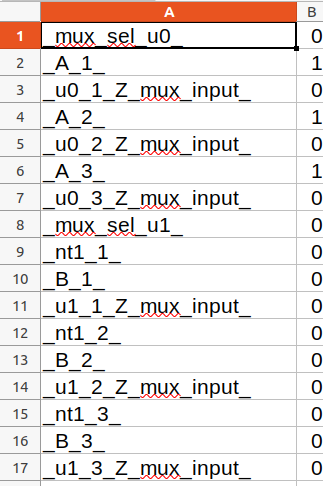
\includegraphics[height=8cm]{figures/csv1.png}
\caption{نمایش خروجی unmapper در نرم‌افزار \lr{LibreOffice Calc}}
\label{fig:csv}
\end{figure}

\end{document}
